\documentclass[12pt]{article}
\usepackage{amsfonts}
\usepackage{fancyhdr}
\usepackage[a4paper, top=2.5cm, bottom=2.5cm, left=2.2cm, right=2.2cm]{geometry}
\usepackage{times}
\usepackage{amsmath}
\usepackage{changepage}
\usepackage{amssymb}
\usepackage{graphicx}%
\setcounter{MaxMatrixCols}{30}
\newtheorem{theorem}{Theorem}
\newtheorem{acknowledgement}[theorem]{Acknowledgement}
\newtheorem{algorithm}[theorem]{Algorithm}
\newtheorem{axiom}{Axiom}
\newtheorem{case}[theorem]{Case}
\newtheorem{claim}[theorem]{Claim}
\newtheorem{conclusion}[theorem]{Conclusion}
\newtheorem{condition}[theorem]{Condition}
\newtheorem{conjecture}[theorem]{Conjecture}
\newtheorem{corollary}[theorem]{Corollary}
\newtheorem{criterion}[theorem]{Criterion}
\newtheorem{definition}[theorem]{Definition}
\newtheorem{example}[theorem]{Example}
\newtheorem{exercise}[theorem]{Exercise}
\newtheorem{lemma}[theorem]{Lemma}
\newtheorem{notation}[theorem]{Notation}
\newtheorem{problem}[theorem]{Problem}
\newtheorem{proposition}[theorem]{Proposition}
\newtheorem{remark}[theorem]{Remark}
\newtheorem{solution}[theorem]{Solution}
\newtheorem{summary}[theorem]{Summary}
\usepackage{enumitem}
\usepackage[utf8]{inputenc}
\newenvironment{proof}[1][Proof]{\textbf{#1.} }{\ \rule{0.5em}{0.5em}}
\usepackage{tikz}
\usetikzlibrary{positioning}
\usepackage{graphicx}
\usepackage{wrapfig}
\usepackage{float}
\usepackage{datetime}
\newdateformat{specialdate}{\twodigit{\THEDAY}.\twodigit{\THEMONTH}.\THEYEAR}
\usepackage{amssymb}
\usepackage{ifsym}
\usepackage{mathtools}
\usepackage{listings}
\usepackage{lipsum}  

\newcommand{\Q}{\mathbb{Q}}
\newcommand{\R}{\mathbb{R}}
\newcommand{\C}{\mathbb{C}}
\newcommand{\Z}{\mathbb{Z}}
\renewcommand\labelenumii{\theenumi.\arabic{enumii}.}

\begin{document}
	
	\title{2. Exercise}
	\author{Timo Bergerbusch 344408 \\ Thomas Näveke 311392 \\ Shu Xing 381176}
	\date{\specialdate\today}
	\maketitle
	
	\section{Exercise 2.1}
	\begin{enumerate}[label=2.1.\arabic*]
		\item \begin{definition}[relational completeness]
			A query language is relationally complete if it is at least as expressive as relational algebra.
		\end{definition}
		Methods with Example table A(\underline{$x_1$},$y_1$) and B(\underline{$y_1$}) \\
		\hspace*{-1cm}\begin{tabular}[c]{l | l | l | l}
			method & RA (Example) & keyword &SQL(Example) \\ \hline \hline
			selection & $\sigma_{x_1 > 0}(A)$ & WHERE &SELECT * FROM A WHERE A.$x_1$ $>$ 0 \\
			projection & $\pi_{x_1}(A)$ & SELECT &SELECT $x_1$ FROM A \\
			cartesian product & A $\times$ B & FROM, CROSS& SELECT * FROM A, B \\
			union & $\sigma_{x_1 > 0}(A) \cup$ & UNION & SELECT * FROM A WHERE $x_1$ $>$ 0 UNION \\
			& $\sigma_{x_1 < 0}(A)$ & & SELECT * FROM A WHERE $x_1$ $<$ 0  \\
			difference & A - A & EXCEPT, NOT IN& SELECT * FROM B WHERE $y_1$ NOT IN A \\
		\end{tabular}
		\item \textbf{1. Beispiel}\\
			  SELECT SUM(salary) FROM works;\\\\
			  \textbf{2. Beispiel}\\
			  SELECT COUNT(city) FROM located; 
		\item Solution Graph:
			\begin{figure}[H]
				\centering
				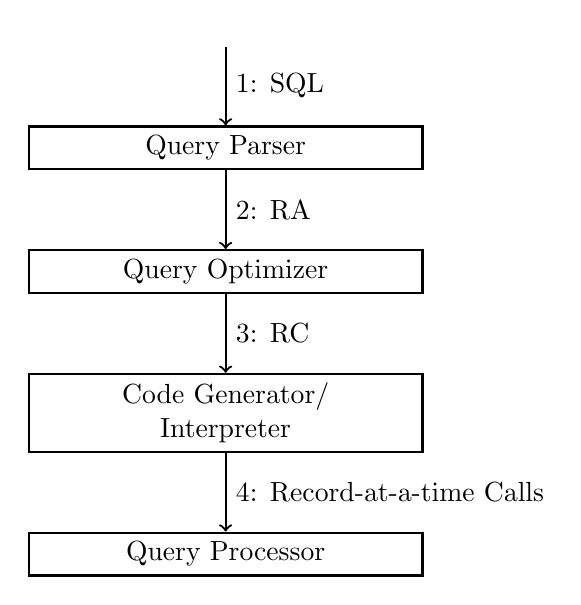
\begin{tikzpicture}
					\node[] (zero) at (0,0) {};
					\node[draw,rectangle, thick, minimum width=5cm, align = center, below = 1cm of zero] (a) {Query Parser};
					\node[draw,rectangle, thick, minimum width=5cm, align = center,below = 1cm of a] (b) {Query Optimizer};
					\node[draw,rectangle, thick, minimum width=5cm, align = center,below = 1cm of b] (c) {Code Generator/ \\ Interpreter};
					\node[draw,rectangle, thick, minimum width=5cm, align = center,below = 1cm of c] (d) {Query Processor};
					
					\draw[thick, ->] (zero) -- (a) node[anchor = west, pos = 0.5] (x1) {1: SQL};
					\draw[thick, ->] (a) -- (b) node[anchor = west, pos = 0.5] (x1) {2: RA};
					\draw[thick, ->] (b) -- (c) node[anchor = west, pos = 0.5] (x1) {3: RC};
					\draw[thick, ->] (c) -- (d) node[anchor = west, pos = 0.5] (x1) {4: Record-at-a-time Calls};
				\end{tikzpicture}						
			\end{figure}
		\item Overview:
			\begin{figure}[H]
				\centering
				\begin{tabular}[c]{l | l}
					operator & operation type \\ \hline \hline
					selection & unary operator \\
					projection & unary operator \\
					cartesian product & set \& binary operator \\
					union & set \& binary operator \\
					difference & set \& binary operator \\
				\end{tabular}				
			\end{figure}
	\end{enumerate}

	\section{Exercise 2.2}
	\begin{enumerate}[label = 2.2.\arabic*]
		\item %maybe same company test?
			\textbf{relational algebra}: \\
			$\pi_{pname}( \rho_{p}(works) \bowtie_{p.cname = b.cname \land p.salary > b.salary}$ \\
			\hspace*{2cm}$ \rho_{b}(works \bowtie_{works.pname = boss.mname} \rho_{pname1\leftarrow pname}(boss) ) )$ \\
			\textbf{tuple relational calculus}:\\
			$\{ <w.pname> \mid w \in works \land \exists m \in boss (w.pname = m.pname \land \exists w^\prime \in works ( w^\prime.pname =m.pname \land w.cname = w^\prime.cname \land w.salary > w^\prime.salary ))  \}$ \\
			\textbf{domain relational calculus}: \\
			$\{ pname \mid \exists cname, salary1, salary2,mname \land works(pname,cname,salary1) \land works(mname, cname, salary2) \land boss(pname, cname) \land salary1 > salary2\}$
		\item 
			\textbf{relational algebra}:\\
			$\pi_{pname}( \rho_{c_1}(works) \bowtie_{c_1.pname=c_2.pname \land c_1.cname != c_2.cname} \rho_{p_2}(works) )$ \\
			\textbf{tuple relational calculus}:\\
			$\{ <w_1.pname> \mid w_1\in works \land \exists w_2 \in works( w_1.pname=w_2.pname \land w_1.cname \neq w_2.cname) \} $ \\
			\textbf{domain relational calculus}:\\
			$\{ pname \mid \exists cname_1, cname_2, salary_1, salary_2 \land works(pname, cname_1, salary_1) \land$ \\
			\hspace*{2cm}$ works(pname, cname_2, salary_2) \land cname_1 \neq cname_2 \} $ \\
		\item 
			\textbf{relational algebra}:\\
			$\pi_{pname}(works) - \pi_{pname}(\rho_{p_1}(works) \bowtie_{p_1.salary < p_2.salary} \rho_{p_2}(works))0$ \\
			\textbf{tuple relational calculus}:\\
			$\{ <w_1.pname> \mid w_1 \in works \land \lnot(\exists w_2 \in works(w_1.cname = w_2.cname \land w_2.salary > w_1.salary ))\} $ \\
			\textbf{domain relational calculus}:\\
			$\{ pname \mid \exists cname, salary_1 \land works(pname,cname,salary_1) \land \lnot(\exists pname_2, salary_2 \land works(pname_2,cname,salary_2) \land salary_2 > salary_1  )\} $ \\
		\item 
			\textbf{relational algebra}:\\
			$\pi_{c_1.cname}( \rho_{c_1}(located) \bowtie_{c_1.city \neq c_2.city} \rho_{c_2}(\sigma_{cname='IBM'}(located)) ) $ \\
			\textbf{tuple relational calculus}:\\
			$\{ <c_1.cname> \mid c_1\in located \land \forall c_2\in located (c_2.cname \neq 'IBM' \lor c_1.city \neq c_2.city) \} $ \\
			\textbf{domain relational calculus}:\\
			$\{ cname \mid \exists city \land located(cname, city) \land \lnot located('IBM', city)\}$ \\
	\end{enumerate}

	\section{Exercise 2.3}
	\begin{enumerate}[label=2.3.\arabic*]
		\item with $N=15000$ and $B=8$: $\lceil \frac{N}{B} \rceil \Rightarrow \lceil \frac{15000}{8} \rceil = 1875$
		\item Number of passes given by: $1+\lceil \log_{B-1}\lceil \frac{N}{B} \rceil \rceil$\\
			  with $N=15000$ and $B=8$ $\Rightarrow 1+\lceil \log_{8-1}\lceil \frac{15000}{8} \rceil \rceil$ = $1+\lceil \log_7 1875 \rceil = 5 $
		\item $ 2 = 1+\lceil \log_{B-1}\lceil \frac{15000}{B} \rceil \rceil \Leftrightarrow 1 = \lceil \log_{B-1}\lceil \frac{15000}{B} \rceil \rceil \Leftrightarrow \frac{1}{2}(1+\sqrt{600001}) \le B \Rightarrow 123 \le B$ \\
		So we need at-least 123 Buffer to be able to sort the file in two passes. %TODO: Umformung aufschreiben
		\item Since we only use 2+1 Pages in a Two-Way-Sort: $B=3$ and $N=15000$ \\ $\Rightarrow 1+\lceil \log_{3-1}\lceil \frac{15000}{2} \rceil \rceil = 14$ passes 
			and $ \lceil \frac{15000}{2} \rceil = 7500$ runs
		
	\end{enumerate}
\end{document}

%\textbf{relational algebra}:
%\textbf{tuple relational calculus}:
%\textbf{domain relational calculus}:


















